% ============================================================
%  PTCD Manufacturing Guide  –  Noble Aggie Labs  –  June 2026
%  Standalone document; paste the \chapter* block into the
%  main report in place of the \todo{} placeholder at app:mfg.
% ============================================================

\documentclass[12pt, letterpaper]{report}% "letterpaper" matches US standard paper size.
\setcounter{tocdepth}{3}
% --- PACKAGES: Each one adds a capability to LaTeX ---
% Think of packages like Python imports or C #includes.


% ---------- Page Layout ----------
\usepackage[top=1in,bottom=1in,left=1in,right=1in]{geometry} % geometry lets you set margins. 1-inch all around is standard for reports.
% ---------- Encoding & Fonts ----------
\usepackage[utf8]{inputenc}% Allows special characters (é, ü, °) to be typed directly.
\usepackage[T1]{fontenc} % Ensures proper font encoding in the output PDF. Without this, copy-pasting from the PDF can produce garbled characters.
% ---------- Graphics & Figures ----------
\usepackage{graphicx}% THE core package for inserting images.
% Usage: \includegraphics[width=0.8\textwidth]{filename.png}
\graphicspath{{figures3/}}
\usepackage{float}% Gives you the [H] placement option for figures/tables. [H] means "put it HERE, not where LaTeX thinks is best." Very useful when you need a figure right after the text that references it.
\usepackage{subcaption}% Lets you put multiple images side-by-side in a single figure environment. Example: Figure 3(a) and Figure 3(b) next to each other.
% ---------- Tables ----------
\usepackage{booktabs} % Provides \toprule, \midrule, \bottomrule for professional-looking tables.
% Rule of thumb: NEVER use vertical lines in tables. Use booktabs rules instead.
\usepackage{tabularx}% Adds the tabularx environment, which lets columns auto-expand to fill width. Great for tables that need to span the full page width.
\usepackage{multirow}% Allows cells that span multiple rows in tables.
\usepackage{longtable}% For tables that are too long to fit on one page (like a Bill of Materials).
% ---------- Math ----------
\usepackage{amsmath}% The standard package for equations. Adds align, equation*, etc.
\usepackage{amssymb}% Extra math symbols (e.g., \therefore, \because, \pm).
\usepackage{siunitx}% Proper formatting for SI units.
\sisetup{per-mode=fraction}
\sisetup{exponent-product=\cdot}
\DeclareSIUnit{\fahrenheit}{\textdegree F}
% Usage: \SI{100}{\celsius}, \SI{10000}{psi}, \SI{10}{\centi\meter}
% This ensures consistent unit formatting throughout the document.
% ---------- Bibliography ----------
\usepackage[numbers, sort&compress]{natbib}
% IEEE-style numeric citations: [1], [2,3], [4-7]
% "sort&compress" turns [3,1,2] into [1-3]
% ---------- Cross-Referencing & Links ----------
\usepackage[
	colorlinks=true,
	linkcolor=blue,      % Internal links (sections, figures)
	citecolor=blue,      % Citation links
	urlcolor=blue         % URL links
]{hyperref}
% Makes all references, citations, and URLs clickable in the PDF.
% Set colorlinks=false if you want boxes instead of colored text.
% ---------- Captions ----------
\usepackage[
	font=small,           % Caption text slightly smaller than body
	labelfont=bf,         % "Figure 1:" is bold
	textfont=it            % The caption description is italic
]{caption}% Makes figure/table captions look more professional.
% ---------- Headers & Footers ----------
\usepackage{fancyhdr}% Customizable headers and footers.
\pagestyle{fancy}% Activate the fancy header/footer style.
\fancyhf{}% Clear all default header/footer content.
\fancyhead[L]{\small Team 16 --- Noble Aggie Labs}% Left header: team name.
\fancyhead[R]{\small EME 185}% Right header: course number.
\fancyfoot[C]{\thepage}% Center footer: page number.
\renewcommand{\headrulewidth}{0.4pt}% Thin line under the header. Set to 0pt to remove.
% ---------- Paragraph Formatting ----------
\usepackage{parskip}% Adds space between paragraphs instead of indenting the first line. This is more common in engineering reports than academic papers.
\setlength{\parindent}{0pt}% Explicitly remove paragraph indentation (parskip should handle this, but belt-and-suspenders doesn't hurt for readability).
% ---------- Line Spacing ----------
\usepackage{setspace}
\onehalfspacing% 1.5 line spacing is easier to read and mark up than single spacing. Change to \doublespacing if required.
%-------- For Box diagrams
\usepackage{tikz}
\usetikzlibrary{patterns}
\usetikzlibrary{patterns,intersections}
\usetikzlibrary{arrows.meta, positioning}
\usetikzlibrary{shapes.geometric}
\usetikzlibrary{arrows.meta, shapes.geometric, shapes.misc, positioning}
\usetikzlibrary{calc}
% ---------- Appendix Support ----------
\usepackage[title,titletoc,page]{appendix} % Adds "Appendices" header and includes appendices in the Table of Contents. [title, titletoc] ensures they are labeled A, B, C
%----------- Title/Chapter formatting -----------------
\usepackage{titlesec}
% Format \chapter to look simple (no giant text, no separate page)
\usepackage{pdfpages}
% Allows you to insert entire PDF Pages (e.g., for Gantt charts, concept screening matrices) with \includepdf.
\usepackage{geometry}
%allows you to set margins and page size. 
\usepackage{mdframed}     % warning/note boxes
\usepackage{enumitem}     % list formatting
\usepackage{booktabs}     % tables
\usepackage{xcolor}       % color support
\usepackage{upgreek}


\definecolor{warnred}{RGB}{180,30,30}
\definecolor{warnbg}{RGB}{255,235,235}
\definecolor{notebg}{RGB}{235,245,255}
\definecolor{noteblue}{RGB}{30,80,160}
\definecolor{ucdgold}{RGB}{207, 184, 124}
\definecolor{ucdblue}{RGB}{0, 40, 85}
\definecolor{sandiablue}{RGB}{0,  174, 214}



\newmdenv[
  linecolor=warnred, backgroundcolor=warnbg,
  linewidth=1.5pt, innerleftmargin=10pt,
  innerrightmargin=10pt, innertopmargin=8pt,
  innerbottommargin=8pt, skipabove=10pt, skipbelow=6pt
]{warningbox}

\newmdenv[
  linecolor=noteblue, backgroundcolor=notebg,
  linewidth=1pt, innerleftmargin=10pt,
  innerrightmargin=10pt, innertopmargin=8pt,
  innerbottommargin=8pt, skipabove=10pt, skipbelow=6pt
]{notebox}


\titleformat{\chapter}
 {\LARGE\bfseries}  % format
 {}                % label
 {0em}                         % sep between label and title
 {}                            % before-code
\titlespacing*{\chapter}{0pt}{20pt}{10pt}  % left, before, after


\makeatletter
\g@addto@macro\appendix{%
 \titleformat{\chapter}[block]
	{\huge\bfseries\centering}
	{\appendixname\ \thechapter}
	{0em}
	{\vspace{0.5em}\\}%
}
\makeatother

% ---------- PDF Metadata ----------
\hypersetup{
    pdftitle={Final Design Report -- Passive Temperature Compensation Device},
    pdfauthor={Team 16: Noble Aggie Labs},
    pdfsubject={EME-185A/B Senior Design, UC Davis}
}
%-----------For landscape pages----------
\usepackage{pdflscape}
\usepackage{pgfplots}
	\pgfplotsset{compat=1.18}
	\usepgfplotslibrary{fillbetween}
	\pgfmathdeclarefunction{normalpdf}{3}{%
    \pgfmathparse{1/(#3*sqrt(2*pi))*exp(-(#1-#2)^2/(2*#3^2))}%
	}
\usepackage{multirow}
\usepackage{array}      % for >{\raggedright\arraybackslash}
\usepackage{makecell}   % for \makecell
\usepackage{calc}
\usepackage{multicol}
\usepackage{mdframed}
\usepackage{wrapfig}

% In your preamble
\newcounter{mycounter}           % creates a counter, initialized to 0
\newcounter{sub}[mycounter]      % resets 'sub' when 'mycounter' increments
% ============================================================================
% SECTION 0.5: CUSTOM COMMANDS (Modular Helpers)
% ============================================================================
% These are reusable shortcuts. Define them once, use them everywhere.
% If a name or term changes, you only edit it in ONE place.


% --- Project-specific shortcuts ---
\newcommand{\projecttitle}{Passive Temperature Compensation Device}
\newcommand{\teamname}{Noble Aggie Labs}
\newcommand{\teamnumber}{16}
\newcommand{\sponsor}{Dr.\ Bradley Bon}
\newcommand{\organization}{Sandia National Laboratories}
\newcommand{\coursename}{EME 185}
\newcommand{\instructor}{Professor Jonathan Schofield}
\newcommand{\university}{University of California, Davis}
\newcommand{\ta}{Teaching Assistant Xiangpu Wang}
\newcommand{\duedate}{5 June 2026}
% --- Convenience commands for common terms ---
% Using these ensures consistent terminology throughout the report.
\newcommand{\device}{PTCD}
\newcommand{\degC}{^{\circ}\text{C}}    % Degree Celsius symbol, properly formatted
\newcommand{\requiredRelationship}{D_{\text{effective}} = A_1 (T_{\text{ambient}} - T_{\text{reference}}) + A_0}
\newcommand{\transferFunction}{D_{\text{eff}}=\frac{dD_{\text{eff}}}{dX} \left[\frac{dL}{dT}\frac{dX}{dL}(T-T_{\text{ref}})+X\left(T_{\text{ref}} \right) \right]}

\newcommand{\Dcoldval}{}
\newcommand{\Dcold}{D_{\text{effective}}(\SI{-60}{\celsius}) = 383.5 \pm \SI{19.2}{\micro\meter}}
\newcommand{\Dhot}{D_{\text{effective}}(\SI{80}{\celsius}) = 170.2 \pm \SI{16.9}{\micro\meter}}
\newcommand{\Dref}{D_{\text{effective}}(\SI{25}{\celsius}) = 292.1 \pm \SI{12.7}{\micro\meter}}

\newcommand{\Thot}{\SI{80}{\degreeCelsius}} %Celcius
\newcommand{\Tcold}{\SI{-60}{\degreeCelsius}} %Celcius
\newcommand{\Tref}{\SI{25}{\degreeCelsius}} %Celcius
\newcommand{\specTempChange}{\SI{140}{\degreeCelsius}}

\newcommand{\specEAl}{\SI{68.95}{\giga \pascal}}
\newcommand{\specEALLV}{\SI{55}{\giga \pascal}}
\newcommand{\specEInv}{\SI{141}{\giga \pascal}}
\newcommand{\specEInc}{\SI{200}{\giga \pascal}}
\newcommand{\specActuatorCTE}{\SI{22.85}{\micro\meter\per\meter\per\celsius}} %Evaluated at 25C
\newcommand{\specMountCTE}{\SI{-30}{\micro\meter\per\meter\per\celsius}}
\newcommand{\specInvarCTE}{\SI{1.3}{\micro\meter\per\meter\per\celsius}}
\newcommand{\specInconelCTE}{\SI{13.2}{\micro\meter\per\meter\per\celsius}}
\newcommand{\specBellowsK}{\SI{75.3}{\kilo \newton \per \meter}} % 430 lb/in
\newcommand{\specBellowsHeight}{\SI{22.86}{\milli \meter}} % = Neck 1 length + Neck 2 length + Conv free diameter = 2*(0.07") + 0.76"
\newcommand{\specBellowsOD}{\SI{6.528}{\milli \meter}} % Conv OD 0.257"
\newcommand{\specBellowsID}{\SI{3.353}{\milli \meter}} % Conv ID 0.132"
\newcommand{\specBellowsSquirm}{\SI{20.68}{\mega \pascal}} % 3000 psi
\newcommand{\specBellowsBurst}{\SI{74.12}{\mega \pascal}} % 10750 psi

\newcommand{\Xhot}{\SI{480.696}{\micro \meter}}
\newcommand{\Xcold}{\SI{213.289}{\micro \meter}}
\newcommand{\specLengthChange}{\SI{267.407}{\micro \meter}}
\newcommand{\govErrorProp}{u_x = \sqrt{\frac{\pi(\sigma_x^2+\sigma_y^2)}{2}}}
\newcommand{\govActuator}{\Delta L = L_0 \Delta T \alpha}
\newcommand{\govValve}{D_{\text{eff}} = \sqrt{\frac{2}{\pi}}}
\newcommand{\specPressure}{\SI{68.95}{\mega \pascal}}%  68.94757 MPa
\newcommand{\AoneExact}{\SI{-1.524e-3}{\milli\meter\per\celsius}}
\newcommand{\Aone}{\AoneExact \pm 5\%}
\newcommand{\AzeroExact}{\SI{0.254}{\milli\meter}}
\newcommand{\Azero}{\AzeroExact \pm 5\%}
\newcommand{\imageHeight}{4in} % Default image height for figures. Adjust as needed.
\newcommand{\specCrossSectArea}{\SI{6.3e-5}{\meter \squared}}
\newcommand{\specOrigActuatorLength}{\SI{32.991}{\milli \meter}}
\newcommand{\specActDefTotal}{\SI{267}{\micro \meter}}
\newcommand{\specActDefHot}{\SI{152.8}{\micro \meter}}

% TF Force Balance Matrix (given as an escaped command because it is given twice in the report)

\newcommand{\forceMatrix}
{
	\begin{bmatrix}
		k_M & k_A  & 0    & 0     & 0     & 0     & 0     & 0     \\
		0   & k_A  & -k_S & 0     & 0     & 0     & 0     & 0     \\
		k_M & 0    & 0    & 0     & 0     & 0     & 0     & -k_W  \\
		0   & 0    & 0    & -k_T  & 0     & 0     & -k_H  & k_W   \\
		0   & 0    & 0    & 0     & -k_B  & k_V   & 0     & 0     \\
		0   & 0    & 0    & 0     & k_B   & 0     & k_H   & 0     \\
		1   & -1   & -1   & 1     & 0     & 0     & 0     & 1    \\
		0   & 0    & 0    & 1     & 1     & 1     & -1    & 0
	\end{bmatrix}
	\begin{bmatrix}
		L_M \\ L_A \\ L_S \\ L_T \\ L_B \\ L_V \\ L_H \\ L_W
	\end{bmatrix}
	=
	\begin{bmatrix}
		k_M \ell_M + k_A \ell_A \\
		k_A \ell_A - k_S \ell_S \\
		k_M \ell_M - k_W \ell_W \\
		k_W \ell_W - k_T \ell_T - k_H \ell_H \\
		k_V \ell_V - k_B \ell_B \\
		k_H \ell_H + k_B \ell_B \\
		0 \\
		0
	\end{bmatrix}
}

% Req and Spec commands
% Offloaded to another document to possibly save the specs as figures if we can't fix the page-break overlap.
% Transfer function specifications

\newcommand{\GA}{\SI{1.91}{\micro\meter\per\celsius}}
\newcommand{\GV}{\num{-0.798}}

% System Requirements
% \newcommand{\ReqA}
% 	{
% 	The device shall passively restrict gas flow according to the Required Relationship
% 	$D_{eff} = A_1 (T_{amb} - T_{ref}) + A_0$
% 	where
% 	\begin{align*}
% 		&D_{eff} \text{ is the effective orifice diameter}
% 		\\
% 		&T_{amb} \text{ is the external ambient temperature}
% 		\\
% 		&T_{ref} = 25 \degC
% 		\\
% 		&A_1 = \Aone
% 		\\
% 		&A_0 = \Azero
% 	\end{align*}
% 	}
\newcommand{\ReqA}{The device shall passively restrict gas flow according to the Required Relationship $D = A_1 \Delta T + A_0$}
\newcommand{\ReqB}{The device should remain within a \SI{10}{\centi\meter} $\times$ \SI{10}{\centi\meter} $\times$ \SI{10}{\centi\meter} mechanical envelope}
\newcommand{\ReqC}{The device shall restrict Hydrogen at \specPressure\ and $T_{amb} + 20 \degC$ for 60 seconds in compliance with requirement R.1}
\newcommand{\RRfull}
{
	\begin{align*}
		D_{eff} &= \hat{G}_{V_0} \hat{G}_{A_0} \Delta T + D_{ref} \\
		&= \frac{dD}{dL} \frac{dL}{dT} (T_{amb} - T_{ref}) + D(T_{ref}) \\
		&= A_1 \Delta T + A_0
	\end{align*}
}

% Valve specifications
\newcommand{\SpecVAA}{The valve subsystem shall passively control the effective orifice diameter as directly driven by the actuator at a conversion rate of $\frac{dD}{dL} = \GV$}
\newcommand{\SpecVAB}{The valve subsystem shall define the reference effective orifice diameter}
\newcommand{\SpecVABapp}{$D_{eff}(T_{ref}) = \AzeroExact$}
\newcommand{\SpecVB}{The valve subsystem shall not exceed a \SI{10}{\centi\meter} $\times$ \SI{5}{\centi\meter} $\times$ \SI{10}{\centi\meter} mechanical envelope}
\newcommand{\SpecVCA}{The housing shall withstand an internal pressure of \specPressure}
\newcommand{\SpecVCB}{Wetted components shall maintain a hermetic seal at an internal pressure of \specPressure}
\newcommand{\SpecVCC}{Wetted components shall not permit Hydrogen diffusion or embrittlement}

% Actuator specifications
\newcommand{\SpecAAA}{The actuator subsystem shall passively drive the valve subsystem in response to ambient temperature at a rate of $\frac{dL}{dT} = \GA$}
\newcommand{\SpecAAB}{The actuator subsystem shall facilitate user calibration of the device}
\newcommand{\SpecAB}{The actuator subsystem shall not exceed a \SI{10}{\centi\meter} $\times$ \SI{5}{\centi\meter} $\times$ \SI{10}{\centi\meter} mechanical envelope}
\newcommand{\SpecACA}{The actuator shall allow no more than \todo{Spec Temp} deviation in its temperature from $T_{amb}$\ within the test window}


% --- Figure insertion helper ---
% This command simplifies inserting a figure with a caption and label.
% Usage: \insertfigure{width}{filename}{caption text}{fig:label}
%
% Parameters:
%   #1 = width relative to text width (e.g., 0.8 for 80%)
%   #2 = filename (without path if images are in the same directory)
%   #3 = caption text
%   #4 = label for cross-referencing (use fig:prefix by convention)
\newcommand{\insertfigure}[4]{%
	\begin{figure}[H]
		\centering
		\includegraphics[width=#1\textwidth]{#2}
		\caption{#3}
		\label{#4}
	\end{figure}
}

% --- TODO marker for draft mode ---
% Prints a bold red "TODO" so you can easily spot incomplete sections.
\usepackage{xcolor}
\usepackage{tocloft} % For listoftodos
% --- TODO marker ---
\newlistof{todos}{tod}{List of TODO's}
\newcommand{\todo}[1]{%
    \textbf{\textcolor{red}{[TODO: #1]}}%
    \addcontentsline{tod}{todos}{\protect\numberline{\thepage}#1}%
}

% For links to spec table
\newcommand{\specref}[1]{\hyperref[tab:specs]{#1}}









\newcommand{\placeholderfig}[3]{%
	\begin{figure}[H]
		\centering
		\fbox{\parbox{#1\textwidth}{\centering\vspace{1.5cm}
			\textit{[Figure placeholder]}\\[4pt]
			\small #2
			\vspace{1.5cm}}}
		% \includegraphics[width=#1\textwidth]{FILENAME}
		\caption{#2}
		\label{#3}
	\end{figure}%
}





\begin{document}

\chapter*{Manufacturing Guide}
\addcontentsline{toc}{chapter}{Manufacturing Guide}
\setcounter{section}{0}
\renewcommand{\thesection}{\arabic{section}}

\begin{center}
	{\Large \textbf{Passive Temperature Compensation Device (PTCD)}} \\[4pt]
	Noble Aggie Labs \\
	Revision 1.0 \\
	June 2026
\end{center}

\bigskip

% ──────────────────────────────────────────────────────────────
%  SAFETY NOTICES
% ──────────────────────────────────────────────────────────────

\begin{warningbox}
	\textbf{\large \textcolor{warnred}{CRITICAL SAFETY NOTICE}}

	\medskip
	Manufacture of this device involves \textbf{sharp tools}, \textbf{high temperatures},
	and dangerous assembly processes such as \textbf{electron-beam welding}.
	Failure to follow these instructions may result in \textbf{serious injury or death.}

	\medskip
	\begin{itemize}[leftmargin=1.5em, itemsep=2pt]
		\item All personnel must be trained in their shop's applicable safety protocols before
					beginning any operation in this guide.
		\item \textbf{Machining:} Sharp cutting tools cause severe lacerations. Never reach into
					a spinning workpiece or move your hands near an unguarded cutter. Wear safety
					glasses at all times on the shop floor. Flying chips are a serious eye hazard.
		\item \textbf{Band saw:} Keep fingers clear of the blade at all times. Use a "chicken finger"
					to manipulate small stock. Do not force any cut.
		\item \textbf{Heat treatment:} The annealing furnace operates at temperatures up to
					\SI{1040}{\degreeCelsius}. Wear heat-resistant gloves and a face shield when
					loading, unloading, or working near an open furnace.
					Allow parts to cool for at least three hours before handling.
		\item \textbf{Electron-Beam Welding (EBW):} EBW generates high-voltage X-rays and an
					intense electron beam. Only trained and certified EBW operators may perform
					welding operations. The operator must confirm the vacuum chamber is sealed and
					all radiation interlocks are engaged before initiating any weld.
	\end{itemize}
\end{warningbox}
\newpage
\begin{warningbox}
	\begin{itemize}[leftmargin=1.5em, itemsep=2pt]
		\item \textbf{Electrical Discharge Machining (EDM):} Dielectric fluid is a skin and
					eye irritant and a fire hazard. Wear chemical-resistant gloves. Ensure the machine
					is fully de-energised before accessing the work zone. Properly dispose of spent
					dielectric fluid.
		\item \textbf{General:} Do not work alone on any operation. Wear
					appropriate personal protective equipment (PPE) at all times, including safety glasses, closed-toe shoes, 
					and long pants.
					Do not wear loose clothing or jewellery while in the shop.
	\end{itemize}
\end{warningbox}

\bigskip

% ──────────────────────────────────────────────────────────────
%  SECTION 1  –  INTRODUCTION AND SCOPE
% ──────────────────────────────────────────────────────────────
\section{Introduction and Scope}

This guide details the complete manufacture, assembly, and calibration of the
Passive Temperature Compensation Device (PTCD), a thermomechanical valve that
passively adjusts a microscopic orifice in response to ambient air temperature.


\subsection{Required Tools}

\begin{notebox}
	\textbf{The following tools and machines are required:}
	\begin{itemize}[itemsep=2pt]
		\item Computer-Numeric Control (CNC) mill and lathe that can meet or exceed the dimensional
					tolerancees in Appendix \ref{app:drawings}
		\item Band saw
		\item Annealing/heat-treatment furnace capable of reaching \SI{1040}{\degreeCelsius}
		\item Sinker EDM (Electrical Discharge Machining) capability
		\item Electron-Beam Welding (EBW) capability
		\item Two perpendicular granite surfaces. One surface must have a drilled hole whose center
					is \SI{20}{\milli\meter} from the intersection between the two surfaces. The
					hole must measure at least \SI{3.4}{\milli\meter} in diameter and \SI{5.1}{\milli\meter}
					depth.
		\item New, carbide-steel tools. Note: this is important to properly machine the parts
					made of Invar 36, which work-hardens as it is cut.
					\todo{Specify which bits are needed}
		\item T6 hand screwdriver
		\item Loctite 243 or similar permanent thread sealant
		\item Cutting fluid for all operations
	\end{itemize}
\end{notebox}

\subsection{Coordinate System}

\begin{notebox}
	\textbf{Coordinate convention used throughout this guide:}
	\begin{itemize}[itemsep=2pt]
		\item \textbf{X~(lateral):} points to the right as one looks downstream along the gas flow.
		\item \textbf{Y~(vertical):} points directly upward.
		\item \textbf{Z~(longitudinal):} points upstream along the direction of gas flow.
	\end{itemize}
\end{notebox}

\begin{figure}[h]
	\centering
	\includegraphics[width=.5\textwidth]{Axes_mfg.png}
	\caption{Reference axes}
	\label{fig:mfg:axes}
\end{figure}

% ──────────────────────────────────────────────────────────────
%  SECTION 2  –  PART IDENTIFICATION
% ──────────────────────────────────────────────────────────────
\section{Part Identification}

Before beginning, familiarise yourself with every part using the figures below
and the Bill of Materials in Appendix~\ref{app:BOM}.

\begin{figure}[H]
	\centering
	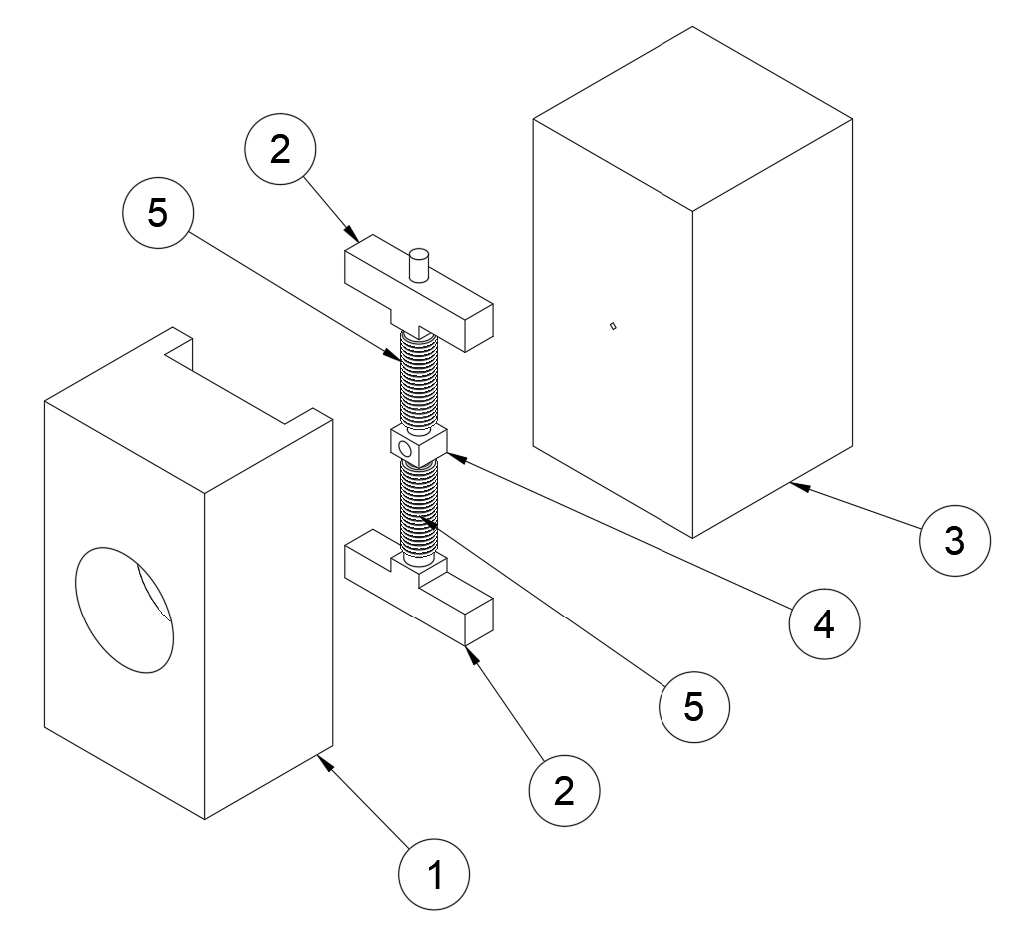
\includegraphics[width=\textwidth]{Valve_ID.png}
	\caption{Valve subsystem part identification}
	\label{fig:valve_ID}
\end{figure}

\begin{figure}[H]
	\centering
	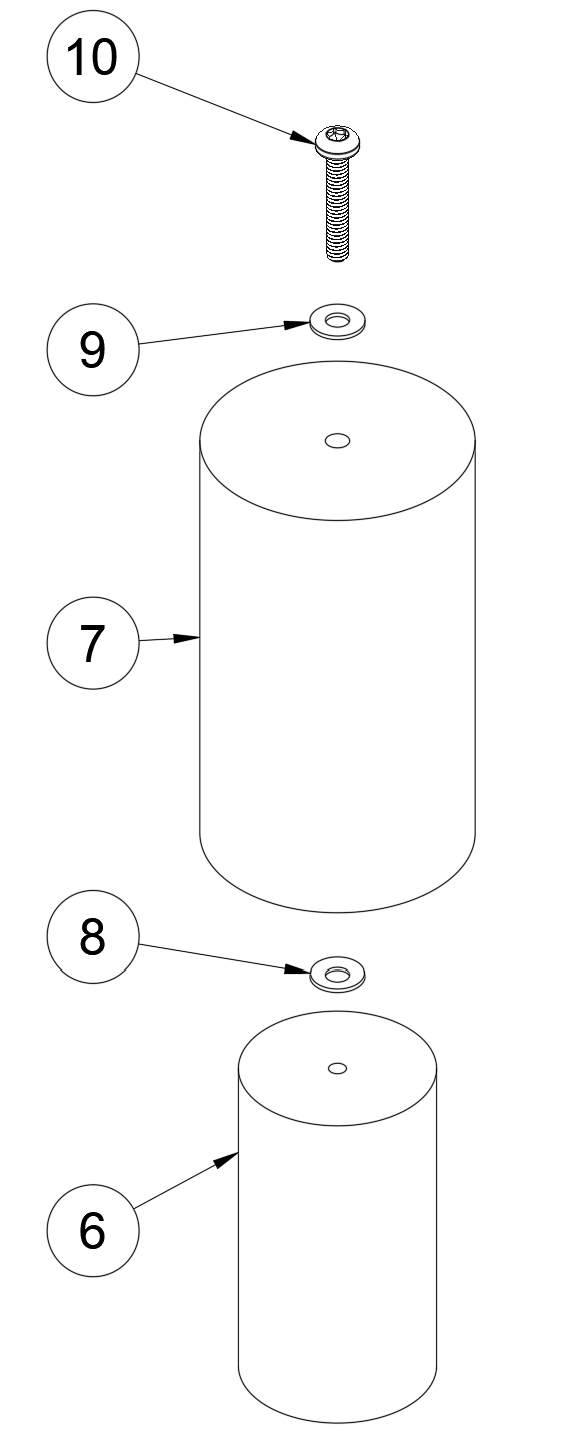
\includegraphics[height=.4\textheight]{Act_ID.png}
	\caption{Actuator subsystem part identification}
	\label{fig:act_ID}
\end{figure}

Table~\ref{tab:mfg_parts} summarises all parts manufactured or purchased for this device.

\begin{table}[H]
	\centering
	\caption{PTCD Bill of Materials summary.}
	\label{tab:mfg_parts}
	\small
	\begin{tabularx}{\textwidth}{llllX}
		\toprule
		\textbf{Part No.} & \textbf{Name} & \textbf{Qty} & \textbf{Material} & \textbf{Source} \\
		\midrule
		V1 & Housing Center   & 2 & Invar 36    & Machined from billet stock \\
		V2 & Housing Inlet    & 1 & Invar 36    & Machined from billet stock \\
		V3 & Housing Outlet   & 1 & Invar 36    & Machined from billet stock \\
		V4 & Valve Orifice    & 1 & Invar 36    & Machined from billet stock \\
		I718-159-72-430 & Bellows & 2 & Inconel 718 & Purchased (Mini-Flex) \\
		A1 & Actuator         & 1 & Al 6061-T6  & Machined from rod stock \\
		A2 & Mount            & 1 & ALLVAR 30   & Machined from rod stock \\
		93237A101 & Belleville Washer & 1 & 316 SS & Purchased (McMaster-Carr) \\
		93475A195 & Standard Washer   & 1 & 18-8 SS & Purchased (McMaster-Carr) \\
		90362A141 & Screw M2$\times$0.4$\times$12 & 1 & 18-8 SS & Purchased (McMaster-Carr) \\
		\bottomrule
	\end{tabularx}
\end{table}

% ──────────────────────────────────────────────────────────────
%  SECTION 3  –  MANUFACTURING
% ──────────────────────────────────────────────────────────────
\newpage
\section{Manufacturing}
\label{sec:mfg}

\subsection{General Machining Notes}
\label{sec:mfg:general}

\begin{notebox}
\textbf{Invar 36 work-hardens during machining.} Use \textbf{new carbide tooling}
throughout. Replace tooling at the first sign of wear; worn tools exacerbate work
hardening and degrade surface finish on critical faces.
\end{notebox}

\textbf{Annealing schedule for all Invar 36 parts:}
\begin{enumerate}[itemsep=2pt]
	\item \textbf{Before machining}: anneal at
				\SI{1040}{\degreeCelsius} (\SI{1900}{\degree F}) for 60~minutes to
				reduce as-received hardness and improve machinability~\cite[p.~6]{ref_Carpenter_Inv}.
	\item \textbf{After all machining is complete}: anneal at
				\SI{93}{\degreeCelsius} (\SI{200}{\degree F}) for 48~hours to relieve
				residual stress and improve long-term dimensional
				stability~\cite[p.~6]{ref_Carpenter_Inv}.
\end{enumerate}
Allow parts to air-cool to room temperature before measuring or proceeding to the
next operation.

\textbf{Referencing convention:}
Before beginning each machining operation, identify which face will serve as the
primary datum. As indicated in the drawings, each of these faces must be carefully
finished to minimize dimensional errors for critical features.

\todo{Bit sizes and orientations for all operations}

% ----------------------------------------------------------
\subsection{Invar 36 Billet Stock: V1, V2, V3, V4}
\label{sec:mfg:invar}
% ----------------------------------------------------------

\textbf{Starting stock:}
44.45~mm $\times$ 76.2~mm $\times$ 82.55~mm
(1\,3/4$''$ $\times$ 3$''$ $\times$ 3\,1/4$''$) Invar 36 billet.
These dimensions will be oriented along the \textbf{lateral (X), vertical (Y), and
longitudinal (Z)} dimensions, respectively.

\begin{warningbox}
\textbf{\textcolor{warnred}{WARNING --- Band Saw Hazard}}
Keep fingers and hands clear of the band saw blade at all times. Use the fence or a
chicken finger to guide stock. Never reach over or behind the blade during a cut. Allow the
blade to come to a complete stop before adjusting the workpiece.
\end{warningbox}

\subsubsection*{Step 1 --- Cross-cut longitudinal axis into blanks}

Using a metal-cutting band saw, cross-cut the longitudinal axis (Z) to produce blanks
of the following \textit{minimum} lengths, leaving additional length for subsequent
facing operations:

\begin{itemize}[itemsep=2pt]
	\item Housing Inlet (V2): \SI{32}{\milli\meter} 
	\item Housing Outlet (V3): \SI{40}{\milli\meter}
	\item Housing Center (V1) / Valve Orifice (V4): \SI{7}{\milli\meter}
\end{itemize}

\begin{notebox}
Account for the band saw blade kerf thickness when planning cut locations.
Typical metal band saw kerfs are \SIrange{1}{2}{\milli\meter} wide. Ensure adequate
additional material remains on each blank after accounting for kerf and facing stock.
\end{notebox}

\subsubsection*{Step 2 --- Cross-cut lateral axis to separate V1 and V4 slugs}

Cross-cut the 7~mm slug along the \textbf{lateral axis (X)} to produce:

\begin{itemize}[itemsep=2pt]
	\item Housing Center $\times$2 (V1): \SI{10}{\milli\meter} lateral length each
	\item Valve Orifice (V4): \SI{7}{\milli\meter} lateral length
\end{itemize}

You now have five rough blanks: V2, V3, two pieces of V1, and V4.

\subsubsection*{Step 3 --- Anneal blanks}

To soften the material before machining the part features,
place all five blanks in the annealing furnace. Anneal at \SI{1040}{\degreeCelsius} for
60~minutes. Allow to air-cool to room temperature before proceeding.

% ------ V1: Housing Center ------
\subsubsection{Housing Center (V1) --- $\times$2}
\label{sec:mfg:V1}

Refer to drawing V1. Produce both Housing Centers identically.

\begin{enumerate}[itemsep=4pt]
	\item \textbf{Mill all six faces} to bring the part to nominal rectangular dimensions.
	\item \textbf{Mill two T-slots on the lateral sides} ($+$X and $-$X faces) for the
				valve orifice sliding interface.
	\item \textbf{Drill through-hole} for the valve stem passage.
				Use a reamer to bring to final H7 tolerance.
\end{enumerate}

% ------ V2: Housing Inlet ------
\subsubsection{Housing Inlet (V2)}
\label{sec:mfg:V2}

Refer to drawing V2.

\begin{enumerate}[itemsep=4pt]
	\item \textbf{Mill all six faces} to nominal rectangular dimensions.
	\item \textbf{Finishing pass on critical faces}
				(the $+$X and $+$Y faces).
				\begin{notebox}
				\textbf{The +X face} is the primary reference for the Housing Inlet.
				Machine this face last among the milled faces, with a dedicated finishing pass
				using a sharp tool at a slow feed rate and light depth of cut.
				The resulting surface must be mirror-smooth; verify with a surface-finish
				gauge or profilometer. This face will be used for critical dimension measurements
				and will be held flush with the corresponding face on the Housing Outlet
				during EBW assembly.
				\end{notebox}
	\item \textbf{Mill top T-groove} on the $+$Y face for the upper valve stem channel.
	\item \textbf{Mill bottom T-groove} on the $-$Y face for the lower valve stem channel.
	\item \textbf{Mill central channel} through the +Z face to form the sliding pocket
				for the Valve Orifice.
	\item \textbf{Drill large central hole}
				through the inlet channel. This is the main gas passage.
	\item \textbf{Drill small inlet hole}
				for the upstream pipe connection.
	\item \textbf{Tap large hole} with G\,3/4-14\,A (in) thread (BSP pipe thread) for
				the upstream pipe fitting. Use a pipe tap and cutting fluid.
\end{enumerate}

% ------ V3: Housing Outlet ------
\subsubsection{Housing Outlet (V3)}
\label{sec:mfg:V3}

Refer to drawing V3.

\begin{enumerate}[itemsep=4pt]
	\item \textbf{Mill all six faces} to nominal dimensions.
	\item \textbf{Finishing pass on Critical Faces A, B, and C}
				(the $+$X, $+$Y, and $+$Z faces respectively).
				\begin{notebox}
				\textbf{The +X and +Y faces} are the primary references for the Housing Outlet.
				Machine these faces last among the milled faces, with a dedicated finishing pass
				using a sharp tool at a slow feed rate and light depth of cut.
				The resulting surfaces must be mirror-smooth; verify with a surface-finish
				gauge or profilometer. These faces will be used for critical dimension measurements
				and will be held flush with the corresponding faces on the Housing Inlet
				during EBW assembly. \\
				\textbf{The +Z face} must be similarly finished to ensure even abuttment against the Housing Inlet.
				\end{notebox}
	\item \textbf{Drill large central hole} as in the Housing Inlet.
	\item \textbf{Plunge small orifice hole} with an end mill.
	\item \textbf{Tap large hole} with G\,3/4-14\,A (in) thread for the downstream
				pipe fitting.
	\item \textbf{Sinker EDM --- square through-orifice:}
				\begin{warningbox}
				\textbf{\textcolor{warnred}{WARNING --- EDM Hazard}}
				The dielectric fluid used in EDM is a fire hazard and a skin/eye irritant.
				Wear chemical-resistant gloves and eye protection. Ensure the EDM machine is
				fully de-energised before accessing the work zone. Dispose of spent fluid per
				facility hazardous-waste procedures.
				\end{warningbox}
				Machine the square through-orifice using sinker EDM.
				Critical requirements:
				\begin{itemize}[itemsep=2pt]
					\item The \textbf{upper interior corner} of the square orifice must have as
								small a fillet radius as possible.
								This is the mission-critical corner; a larger fillet directly degrades
								the effective diameter accuracy.
					\item Minimise EDM recast (white) layer on all orifice edges; no
								micro-cracking is permitted.
					\item Thoroughly clean the part after EDM to remove all dielectric fluid
								and microscopic debris before proceeding.
					\item The horizontal and vertical position of the critical
								upper corner must be held as exactly as possible.
								Verify with optical metrology after EDM.
				\end{itemize}
\end{enumerate}

\begin{notebox}
\textbf{EDM Integrity Verification} \\
Confirmation of the above requirements requires a destructive test.
Perform an identical operation to the one specified on a sample workpiece. Carefully cut
the piece in two along its central axis and optically verify that no EDM recast or
micro-cracking is present.
\end{notebox}

% ------ V4: Valve Orifice ------
\subsubsection{Valve Orifice (V4)}
\label{sec:mfg:V4}

Refer to drawing V4.

\begin{enumerate}[itemsep=4pt]
	\item \textbf{Mill $\pm$Z and $\pm$X faces} to bring part to nominal rectangular
				dimensions.
	\item \textbf{Finish all faces} except for the -Y face, paying especial attention
				to the +X face.
	\item \textbf{Plunge small hole} with an end mill.
	\item \textbf{Sinker EDM --- square through-orifice (leading orifice):}
				Machine the square through-orifice using sinker EDM as per the above EDM operation.
	\item \textbf{TiN PVD coating:} Apply a TiN (titanium nitride) Physical Vapor
				Deposition coating to the four contact surfaces per drawing V4, Note~5.
				Confirm the coating thickness does not exceed \SI{0.004}{\milli\meter};
				re-measure the g6 dimensions after coating and verify the fit is maintained
				before proceeding to assembly.
\end{enumerate}

% ----------------------------------------------------------
\subsection{6061 Aluminum Rod Stock: A1 (Actuator)}
\label{sec:mfg:A1}
% ----------------------------------------------------------

\textbf{Starting stock:}
\O\,\SI{19.05}{\milli\meter} $\times$ \SI{76.2}{\milli\meter}
(\O\,3/4$''$ $\times$ 6$''$) 6061-T6 Aluminum rod.

\begin{enumerate}[itemsep=4pt]
	\item \textbf{Band saw --- cut to length:} Cross-cut the rod to a length slightly
				above nominal; leave material for facing.
	\item \textbf{Mill to length:} Face both $+$Y and $-$Y ends on the milling
				machine to remove band saw marks and bring the part close to nominal length.
	\item \textbf{Finishing pass on $+$Y face (top):}
				\begin{notebox}
				The length of the actuator is a
				\textbf{critical dimension}: it directly sets the actuator expansion rate.
				\end{notebox}
	\item \textbf{Lathe --- turn outside diameter:} Turn the outer diameter.
	\item \textbf{Drill central hole:} Drill the axial hole
				through the top of the part, centred on the axis.
	\item \textbf{Tap:} Tap M2$\times$0.4 6H thread in the central hole for the
				calibration screw.
\end{enumerate}

% ----------------------------------------------------------
\subsection{ALLVAR 30 Rod Stock: A2 (Mount)}
\label{sec:mfg:A2}
% ----------------------------------------------------------

\textbf{Starting stock:}
\O\,\SI{25.4}{\milli\meter} $\times$ \SI{45.72}{\milli\meter}
(\O\,1$''$ $\times$ 1.8$''$) ALLVAR Alloy 30 rod.

\begin{enumerate}[itemsep=4pt]
	\item \textbf{Band saw --- cut to length:} Cross-cut the rod slightly above
				nominal.
	\item \textbf{Mill to length:} Face both ends to remove saw marks and bring to
				near-nominal height.
	\item \textbf{Finishing pass on $-$Y face (bottom):}
				\begin{notebox}
				The $-$Y face is electron-beam welded to the top of the housing. A flat,
				clean surface is essential for the intimate joint
				required by EBW. Machine this face last with a
				light finishing pass. Verify flatness with a surface plate and feeler gauge
				before proceeding.
				\end{notebox}
	\item \textbf{Drill small clearance hole:} Drill
				the center through hole to a minimum depth of \SI{5}{\milli\meter}.
	\item \textbf{Drill large inner hole:}
				Drill the bulk of the large hole. Leave ample diametral and axial clearance for
				precise dimensions.
	\item \textbf{Bore large inner hole:}
				Carefully bore the hole's inner diameter to tolerance.
				Do not bore the entire hole; leave axial clearance at the end to avoid
				damaging the end face.
	\item \textbf{Plunge large inner hole:}
				Plunge the hole with a long end mill. Perform a finishing pass to bring the
				hole's length to tolerance and to square the circumference of its inner face.
	\item \textbf{Turn outer diameter:} turn the outer diameter with a lathe.
\end{enumerate}

% ──────────────────────────────────────────────────────────────
%  SECTION 4  –  ASSEMBLY
% ──────────────────────────────────────────────────────────────
\section{Assembly}
\label{sec:assy}

\begin{warningbox}
\textbf{\textcolor{warnred}{WARNING --- Electron-Beam Welding (EBW) Hazard}}

EBW generates high-voltage X-ray radiation and a focused electron beam.
\textbf{Only trained, certified EBW operators} may perform these operations.
Confirm all radiation interlocks are active and the vacuum chamber is sealed
before initiating any weld. No EBW operation may be performed by untrained
personnel under any circumstances.
\end{warningbox}

\subsection{General Assembly Notes}

All permanent joints in the PTCD, except the actuator-mount connection
secured by the calibration screw,
are made by Electron-Beam Welding (EBW).
EBW requirements (drawing W1, W2 notes) apply to all weld operations:

\begin{enumerate}[itemsep=3pt]
	\item Welding process: EBW (autogenous; no filler metal).
	\item Mating surfaces must be intimate; maximum gap $\leq$\,\SI{0.01}{\milli\meter}.
	\item All surfaces to be welded must be thoroughly cleaned and free of oil, grease,
				and oxidation prior to welding. Use appropriate solvent (e.g.\ isopropyl
				alcohol) and clean-room wipes.
	\item Purge internal cavities with inert gas (e.g.\ argon) during welding to
				prevent oxidation and spatter.
	\item All wetted EBW joints must be subjected to 100\% X-ray radiographic
				examination (RT) to confirm a weld joint efficiency $E = 1.0$ per
				ASME~B31.3~\cite{ref_asme_b313}.
\end{enumerate}

EBW requires an unobstructed line of sight to the weld joint throughout the
full rotation of the workpiece. Plan each setup carefully. The sub-assembly
sequence in Sections~\ref{sec:valve_assy} and~\ref{sec:act_assy} is designed
to maintain 360$^{\circ}$ weld access at every stage.

% ----------------------------------------------------------
\subsection{Valve Sub-Assembly}
\label{sec:valve_assy}
% ----------------------------------------------------------

\begin{notebox}
\textbf{Required tooling for valve assembly:}
\begin{itemize}[itemsep=2pt]
	\item Two perpendicular granite surface plates. One plate must contain a clearance
				hole at least \SI{3.4}{\milli\meter} in diameter and at least \SI{5}{\milli\meter}
				deep at precisely \SI{20}{\milli\meter} from the intersection between the plates
				(to accept the lower valve stem during
				step~\ref{step:lay_granite}).
	\item Clean lint-free gloves and wipes.
	\item Optical comparator or profilometer for verifying face flush and orifice position.
\end{itemize}
\end{notebox}

\begin{figure}[H]
	\centering
	
\includegraphics[width=.5\textwidth]{Valve_exploded.png}
	\caption{Valve subsystem exploded view}
	\label{fig:valve_exploded}
\end{figure}

\subsubsection*{Step 1 --- Weld bellows to Valve Orifice (V4)}

\begin{enumerate}[itemsep=4pt]
	\item Orient the first (upper) bellows with its \textbf{small neck (Neck~1) toward
				the center} of the Valve Orifice. Seat it on the upper valve stem stub of V4.
	\item Orient the second (lower) bellows identically: small neck toward center, seated
				on the lower valve stem stub.
	\item EBW both bellows to V4 with circumferential welds.
\end{enumerate}

\subsubsection*{Step 2 --- Add Housing Centers (V1) to valve stems}
\label{step:add_V1}

\begin{enumerate}[itemsep=4pt]
	\item Slide one Housing Center (V1) onto the upper valve stem of the
				V4--bellows sub-assembly through its bore.
				The V1 piece should slide freely without binding.
	\item Slide the second Housing Center onto the lower valve stem.
\end{enumerate}

\subsubsection*{Step 3 --- Lay sub-assembly on granite surface and tack-weld}
\label{step:lay_granite}

\begin{enumerate}[itemsep=4pt]
	\item Set the sub-assembly on the
				granite surface plate, with the -Z face against the surface.
	\item Apply \textbf{two spot welds} at each bellows--Housing Center connection 
				to fix their position.
\end{enumerate}

\subsubsection*{Step 4 --- Full weld of Housing Centers to bellows}

\begin{enumerate}[itemsep=4pt]
	\item Remove the sub-assembly from the granite surface.
	\item Fully EBW each Housing Center to its bellows with a circumferential weld.
\end{enumerate}

\subsubsection*{Step 5 --- Insert valve sub-assembly into Housing Inlet (V2)}

\begin{enumerate}[itemsep=4pt]
	\item Verify that the V4 coated surfaces are clean and the housing channel in V2 is
				free of debris.
	\item Slide the sub-assembly (V4 + bellows + V1~$\times$2) into the central
				channel of the Housing Inlet (V2).
\end{enumerate}

\subsubsection*{Step 6 --- EBW Housing Centers to Housing Inlet; verify face flush}

\begin{enumerate}[itemsep=4pt]
	\item With the sub-assembly fully seated in V2, EBW the Housing Centers (V1) to
				the Housing Inlet (V2).
\end{enumerate}

\subsubsection*{Step 7 --- Finish the Housing Inlet face}

\begin{enumerate}[itemsep=4pt]
	\item Make a finishing pass across the whole -Z face of the subassembly to
				ensure flush abuttment against the Housing Oulet.
				Be careful not to damage the bellows while cutting.
\end{enumerate}

\subsubsection*{Step 8 --- Connect the Housing Outlet}

\begin{enumerate}[itemsep=4pt]
	\item Invert the assembly and set its +Y and +X faces flush against the two granite surfaces.
				Use the provided hole to make room for the protruding valve stem.
	\item Set the Housing Inlet in like manner against the granite surfaces.
				Butt its +Z face against the assembly's -Z face.
	\item Weld the assembly along its exposed edges enough to secure the parts in place.
				Remove from the granite surfaces; fully weld the connection.
\end{enumerate}

\subsubsection*{Step 9 --- Finish the Upper Surface}

\begin{enumerate}[itemsep=4pt]
	\item Perform a finishing pass on the +Y surface of the assembly.
	Maintain clearance around the valve stem at a minimum of \SI{1}{\milli\meter}
	to avoid damage and a maximum of \SI{7}{\milli\meter} to ensure the full mount-housing
	contact surface is finished.
\end{enumerate}

% ----------------------------------------------------------
\subsection{Actuator Sub-Assembly}
\label{sec:act_assy}
% ----------------------------------------------------------

\begin{figure}[H]
	\centering
	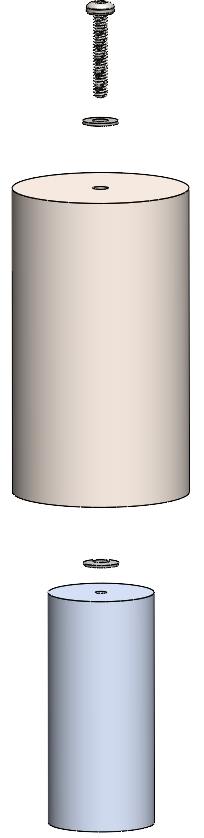
\includegraphics[height=3in]{Act_exploded.png}
	\caption{Actuator subsystem exploded view}
	\label{fig:act_exploded}
\end{figure}

\subsubsection*{Step 1 --- EBW Actuator (A1) to upper valve stem}

\begin{enumerate}[itemsep=4pt]
	\item EBW the actuator to the valve stem.
				Confirm the actuator and valve stem are axially
				aligned; any tilt introduces an off-axis load on the orifice.
\end{enumerate}

\begin{notebox}
\textbf{Thermal equilibration}\\
Before proceeding, allow all parts to thermally equilibriate with their environment for a full
60 minutes. This ensures that the device can be calibrated before the thread lubricant sets.
\end{notebox}

\subsubsection*{Step 2 --- Add Mount and Calibration Assembly}

\begin{enumerate}[itemsep=4pt]
	\item Apply Loctite 243 or a similar lubricant-sealant to the screw.
	\item Invert the mount (A2). Insert the screw (90362A141) through the
				standard flat washer (93475A195) and mount.
				Slide the Belleville washer (93237A101) onto the screw,
				conical side facing toward the mount top when righted.
	\item Invert the housing-actuator assembly. Carefully insert the actuator into the
				the mount until it hits the screw. Thread the screw into the actuator untilthe mount
				can sit flush against the housing and the Belleville washer is slightly compressed.
	\item Right the assembly and EBW the mount to the housing.
\end{enumerate}

\begin{notebox}
\textbf{Time-sensitive calibration}
Perform the calibration steps detailed in Section \ref{sec:calibration} immediately
to ensure the thread sealant does not set.
\end{notebox}

% ──────────────────────────────────────────────────────────────
%  SECTION 5  –  CALIBRATION
% ──────────────────────────────────────────────────────────────
\section{Calibration}
\label{sec:calibration}

Calibrate the \device\ at approximately $T_{ref} = \Tref$ (room temperature).

\subsubsection*{Calibration Procedure}

\begin{enumerate}[itemsep=5pt]
	\item \textbf{Thread the gas supply.} Connect the PTCD to a controlled gas flow
				supply via its threaded interfaces. Precisely measure the ambient temperature
				and the pressure differential across the device.
	\item \textbf{Calculate required pressure drop.} Use the following equations to determine
				the required pressure differential for the current temperature:
				\begin{align}
					D_{\text{effective}} = A_1 (T_{\text{ambient}} - T_{\text{reference}}) + A_0 \\
					A_1 = \Aone \\
					T_{\text{reference}} = \SI{25}{\degreeCelsius} \\
					A_0 = \Azero \\
					A = \frac{\pi}{4} D_{\text{effective}} \\
					Q = C_d A \sqrt{\frac{2 \Delta P}{\rho (1 - \beta^4)}} \label{eq:white}
				\end{align}
				Refer to White's Fluid Mechanics\cite[eq.~6-102]{ref_white} for interpretation of
				equation \eqref{eq:white}.
	\item \textbf{Adjust the orifice.} Using a T6 Torx driver, turn the calibration
				screw in small increments. Turn it clockwise to increase the effective
				diameter and decrease the pressure differential.
	\item \textbf{Depressurise and disconnect.} Let the system run at steady-state for six hours
				to allow the sealant to fully set under these conditions. Then close the supply valve and vent
				the downstream line before disconnecting any fittings.
\end{enumerate}

\end{document}